\par Le membre du groupe responsable de cette partie était Emmanuel Guet.

Dans un jeu de type Shoot'Em, il est évident que les ennemis font partie intégrante du jeu.
C'est pourquoi le travail les concernant a été conséquent, et il en résulte une flopée d'ennemis, dont le rôle diffère réellement d'un ennemi à un autre. Cette partie est là pour tenter de les expliquer au mieux, en donnant quelques statistiques les concernant.

		\begin{itemize}
			\item[$\bullet$ Drone]
				\par~
				\begin{itemize}
					\item Vie : 20
					\item Dommages en cas de collision : Faibles
					\item Vitesse : Rapide
					\item Aptitude : Blaster
					\item Dangerosité : 5%
					\item Rôle : Il s'agit de l'ennemi le moins dangereux, mais aussi de l'ennemi le plus présent. Il ne dispose d'aucune capacité spécifique, et son attaque, un Aptitude au Blaster, n'inflige que peu de dégâts, c'est pourquoi sa dangerosité est si basse.
				\end{itemize}

\includegraphics[width=11cm]{images/vaisseaux/drone.png}
				\par~
			\item[$\bullet$ Double Shooter]
				\par~
				\begin{itemize}
					\item Vie : 40
					\item Dommages en cas de collision : Faibles
					\item Vitesse : Rapide
					\item Aptitude : Blaster ($\times2$)
					\item Dangerosité : 10%
					\item Rôle : Une évolution du Drone. En conséquence, la dangerosité reste basse, toutefois se faire toucher par plusieurs rafales d'affilée implique des dégâts conséquents.
				\end{itemize}
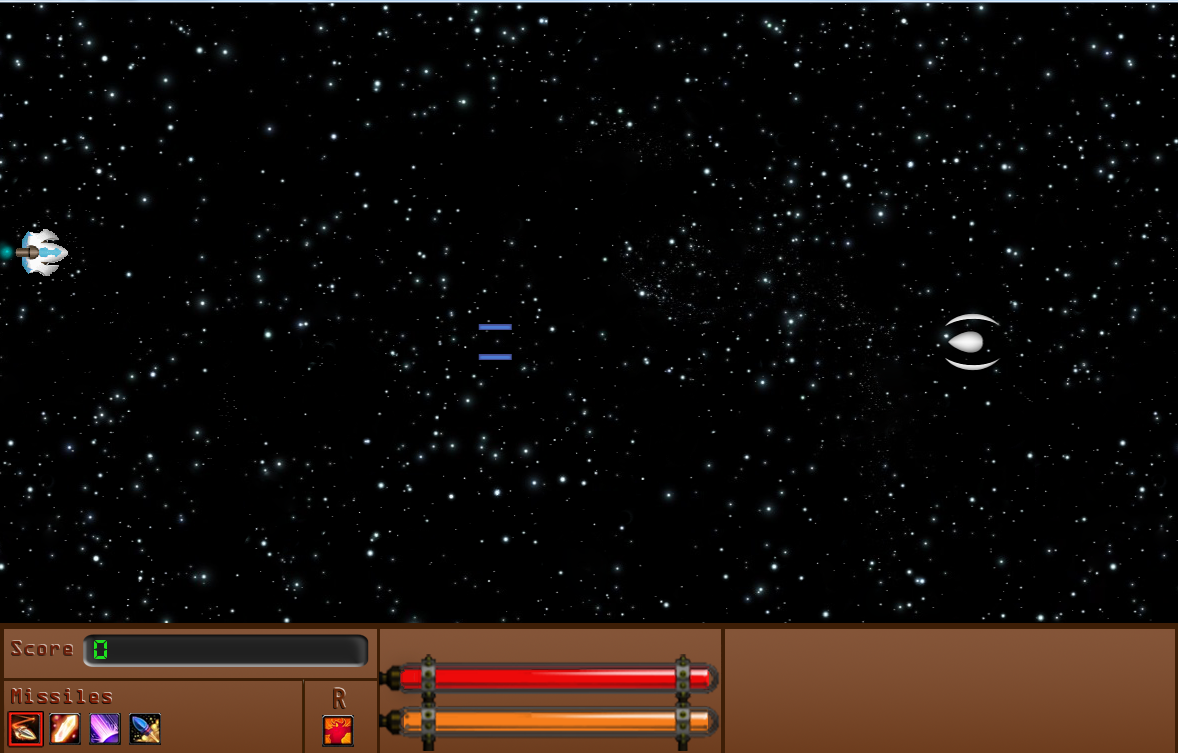
\includegraphics[width=11cm]{images/vaisseaux/doubleshooter.png}
			\item[$\bullet$ Blasterer]
				\par~
				\begin{itemize}
					\item Vie : 50
					\item Dommages en cas de collision : Faibles
					\item Vitesse : Lente
					\item Aptitude : Énergie filée
					\item Dangerosité : 15%
					\item Role : L'ennemi le plus résistant à l'heure actuelle. Il avance lentement, Aptitude à cadence lente avec une arme infligeant des dégâts importants. Il est vital de ne pas subir plusieurs fois de l'énergie filée ...
				\end{itemize}
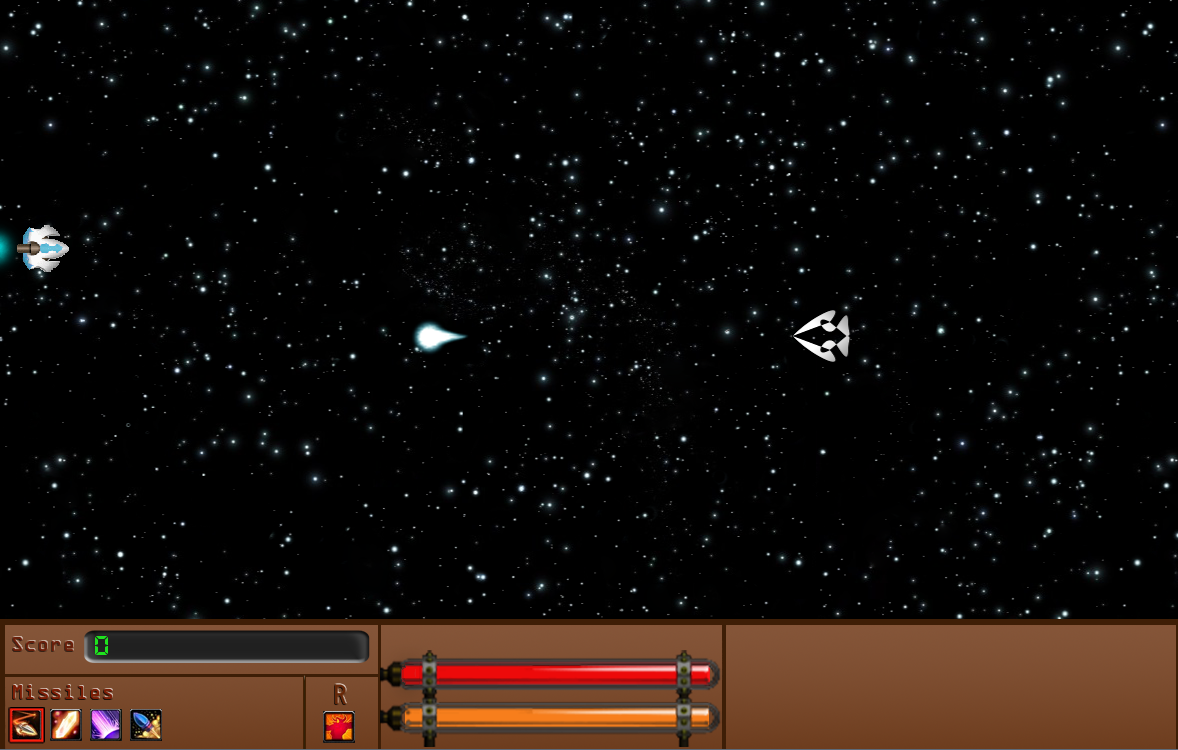
\includegraphics[width=11cm]{images/vaisseaux/blasterer.png}
				\par~
			\item[$\bullet$ Kamikaze]
				\par~
				\begin{itemize}			
					\item Vie : 5
					\item Dommages en cas de collision : Très élevés
					\item Vitesse : Très rapide
					\item Aptitude : Aucun
					\item Dangerosité : 25%
					\item Rôle : Un ennemi très rapide et qui inflige d'énorme dégâts à l'impacte. Tel un kamikaze, il cherche à s'encastrer contre le vaisseau du joueur, lui enlevant ainsi 1/5e de sa vie. Il devient ainsi un ennemi dont le potentiel dangereux commence à devenir important.
				\end{itemize}
				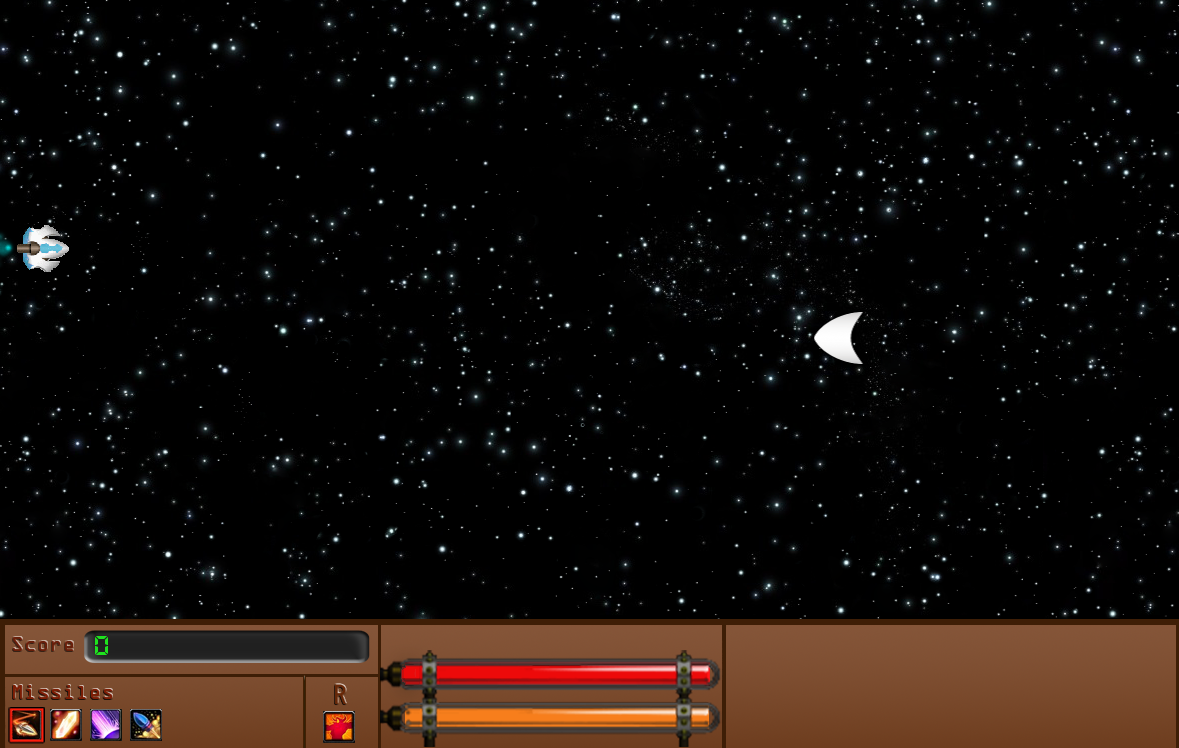
\includegraphics[width=11cm]{images/vaisseaux/kamikaze.png}
				\par~
					\item[$\bullet$ Zebra]
				\par~
				\begin{itemize}
					\item Vie : 5
					\item Dommages en cas de collision : Faibles
					\item Vitesse : Moyenne
					\item Aptitude : Aucun
					\item Dangerosité : 10%
					\item Rôle : Il s'agit d'un ennemi qui bouge de haut en bas dans le niveau. Il est là pour obliger le joueur à augmenter sa vigilance, mais reste un ennemi peu dangereux. Attention toutefois s'il en apparait plusieurs, ils peuvent rapidement devenir dangereux.
				\end{itemize}
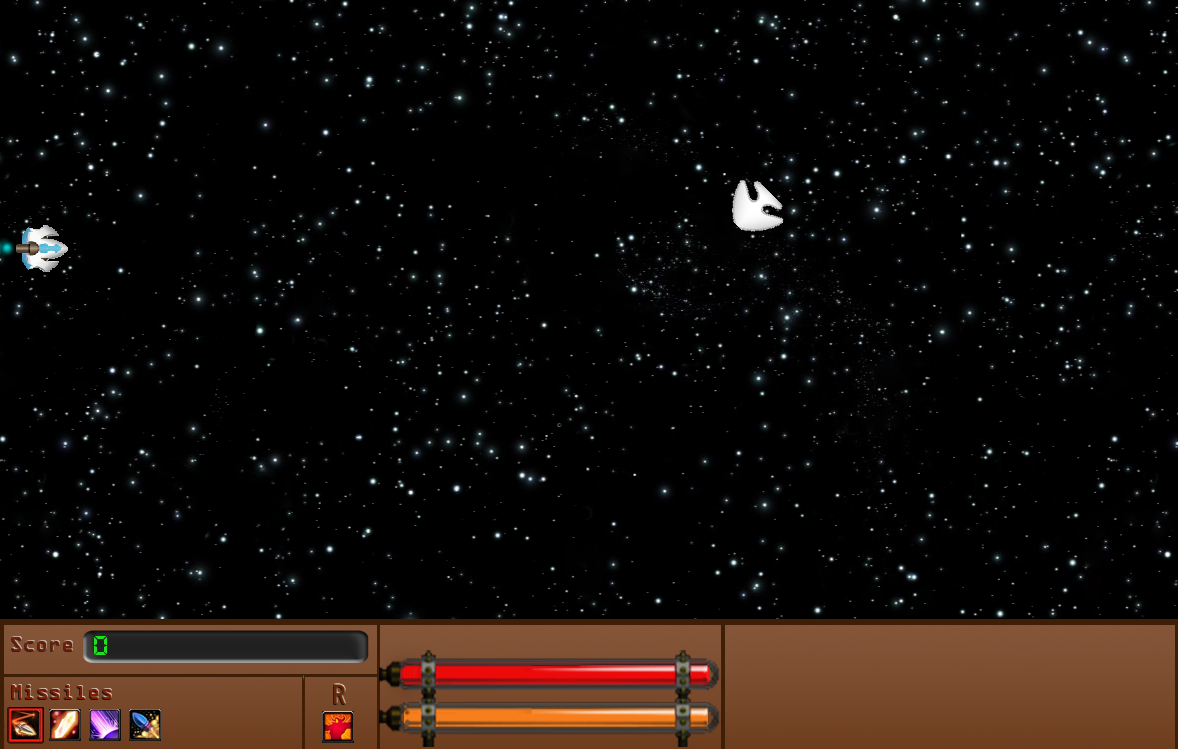
\includegraphics[width=11cm]{images/vaisseaux/zebra.png}
				\par~
				\item[$\bullet$ Battle Cruiser]
				\par~
				\begin{itemize}
					\item Vie : 50
					\item Dommages en cas de collision : Faibles
					\item Vitesse : Moyenne
					\item Aptitude : Chargement du laser - Laser
					\item Dangerosité : 50%
					\item Role : Le premier ennemi réellement dangereux. Il va charger un laser boosté à l'ambodium, une technologie alien, qui permet d'infliger des dégâts incroyablement élevés. De plus, étant invincibles pendant ce chargement, une fois commencé, rien ne peut les arrêter. Faites-attention !
				\end{itemize}
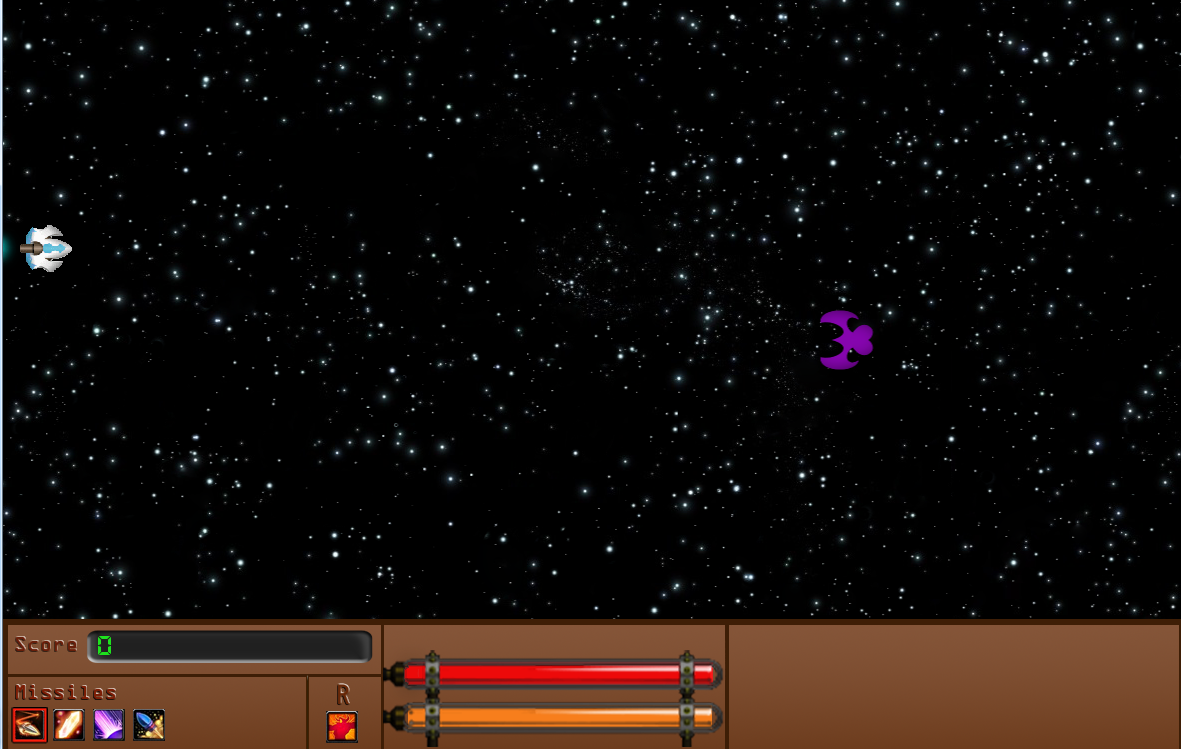
\includegraphics[width=11cm]{images/vaisseaux/bc_load.png}
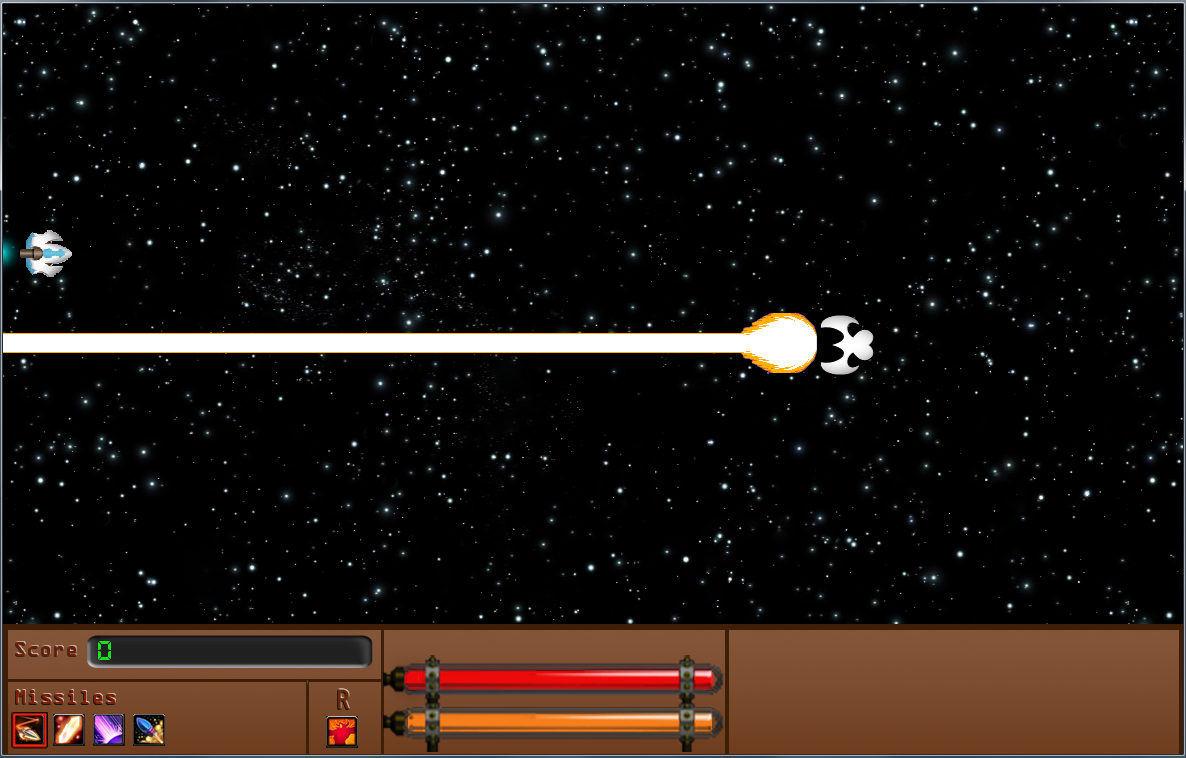
\includegraphics[width=11cm]{images/vaisseaux/bc_fire.png}

				\par~
				\item[$\bullet$ Targeter]
				\par~
				\begin{itemize}
					\item Vie : 50
					\item Dommages en cas de collision : Faibles
					\item Vitesse : Moyenne
					\item Aptitude : Boule d'énergie autoguidée
					\item Dangerosité : 45%
					\item Rôle : Le Targeter a la capacité de pouvoir tirer une boule d'énergie autoguidée, qui va donc suivre le joueur. Le seul moyen de s'en séparer et de s'en rapprocher suffisamment. Adrénaline garantie !
				\end{itemize}

\includegraphics[width=11cm]{images/vaisseaux/targeter.png}
				\par~
				\item[$\bullet$ Support]
				\par~
				\begin{itemize}
					\item Vie : 50
					\item Dommages en cas de collision : Faibles
					\item Vitesse : Très rapide mais s'arrête au milieu de l'écran
					\item Aptitude : Aura généreuse
					\item Dangerosité : 70%
					\item Rôle : Cet ennemi est sans aucun doute le plus dangereux. Et pourtant, il ne possède aucune capacité offensive. Il va s'installer au milieu de l'écran et déployer son aura généreuse, qui divise tous les dégâts infligés par le joueur par 4. La taille de l'aura augmente au fur et à mesure que le support est présent sur le terrain. Attention à ne pas le laisser en vie trop longtemps sous peine de défaite obligatoire !
				\end{itemize}
				\begin{center}
					\par 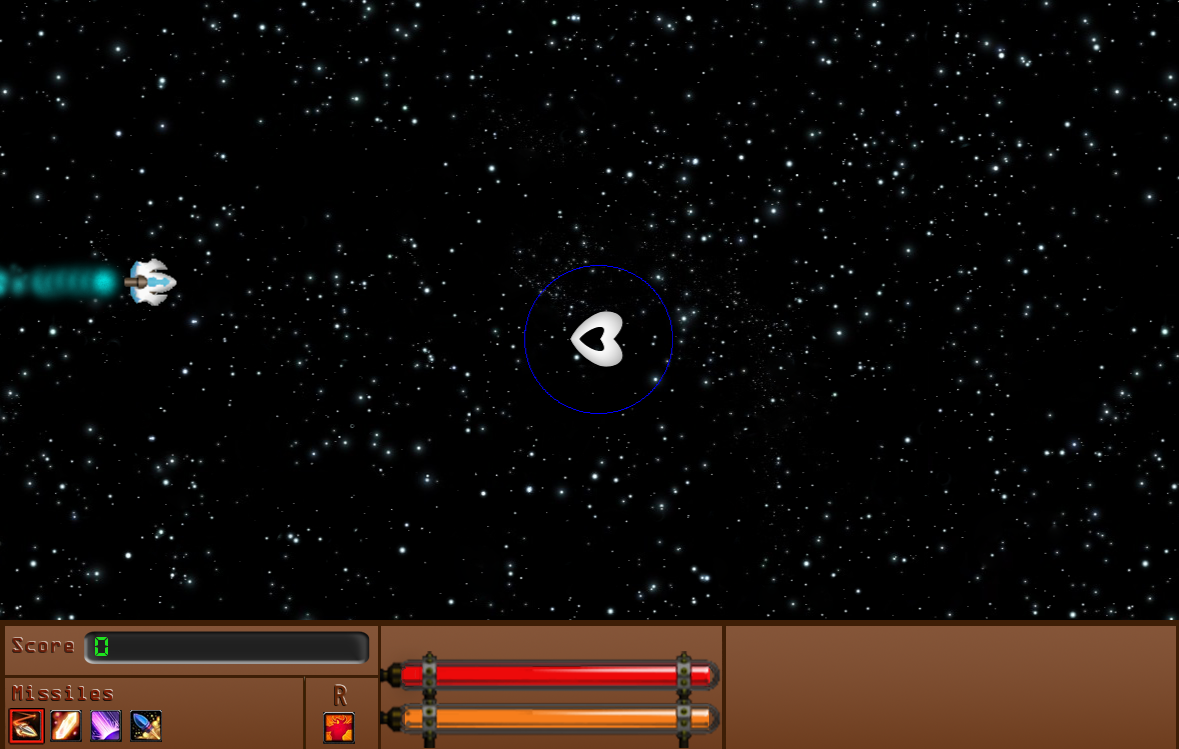
\includegraphics[width=11cm]{images/vaisseaux/support_little.png}
					\par 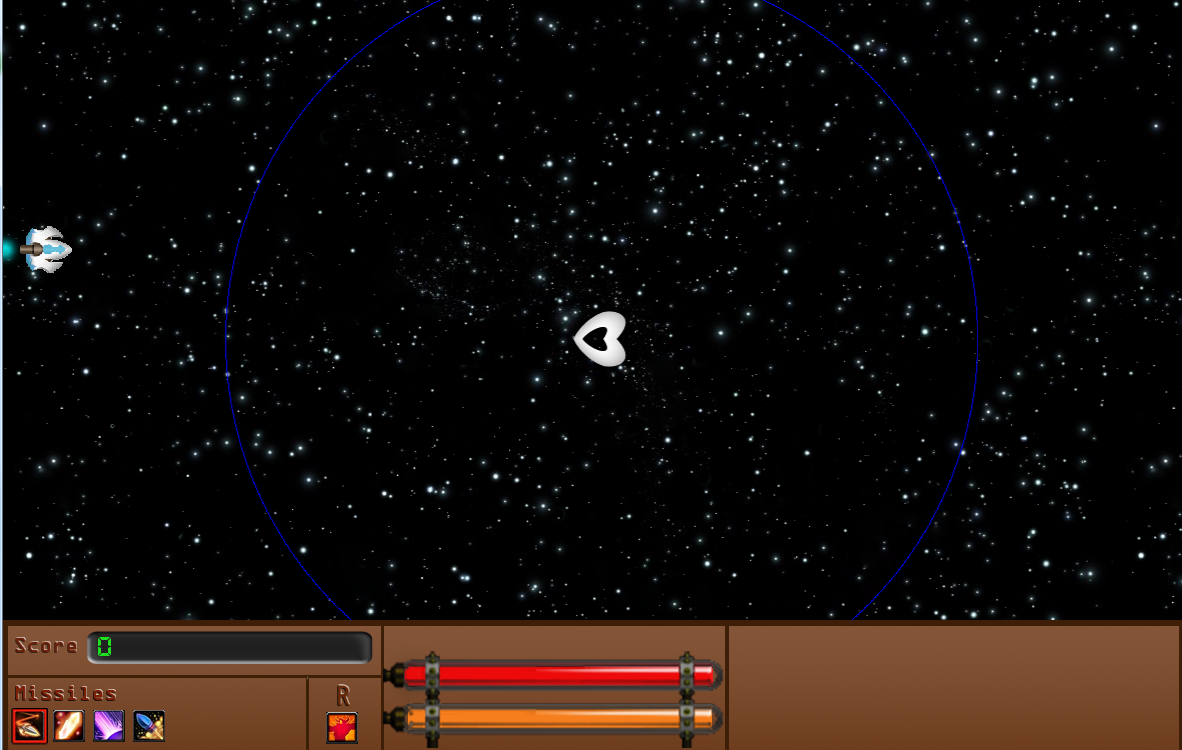
\includegraphics[width=11cm]{images/vaisseaux/support_huge.png}
				\end{center}

				\par~
		\end{itemize}